% Options for packages loaded elsewhere
\PassOptionsToPackage{unicode}{hyperref}
\PassOptionsToPackage{hyphens}{url}
%
\documentclass[
]{article}
\usepackage{amsmath,amssymb}
\usepackage{lmodern}
\usepackage{iftex}
\ifPDFTeX
  \usepackage[T1]{fontenc}
  \usepackage[utf8]{inputenc}
  \usepackage{textcomp} % provide euro and other symbols
\else % if luatex or xetex
  \usepackage{unicode-math}
  \defaultfontfeatures{Scale=MatchLowercase}
  \defaultfontfeatures[\rmfamily]{Ligatures=TeX,Scale=1}
\fi
% Use upquote if available, for straight quotes in verbatim environments
\IfFileExists{upquote.sty}{\usepackage{upquote}}{}
\IfFileExists{microtype.sty}{% use microtype if available
  \usepackage[]{microtype}
  \UseMicrotypeSet[protrusion]{basicmath} % disable protrusion for tt fonts
}{}
\makeatletter
\@ifundefined{KOMAClassName}{% if non-KOMA class
  \IfFileExists{parskip.sty}{%
    \usepackage{parskip}
  }{% else
    \setlength{\parindent}{0pt}
    \setlength{\parskip}{6pt plus 2pt minus 1pt}}
}{% if KOMA class
  \KOMAoptions{parskip=half}}
\makeatother
\usepackage{xcolor}
\usepackage[margin=1in]{geometry}
\usepackage{longtable,booktabs,array}
\usepackage{calc} % for calculating minipage widths
% Correct order of tables after \paragraph or \subparagraph
\usepackage{etoolbox}
\makeatletter
\patchcmd\longtable{\par}{\if@noskipsec\mbox{}\fi\par}{}{}
\makeatother
% Allow footnotes in longtable head/foot
\IfFileExists{footnotehyper.sty}{\usepackage{footnotehyper}}{\usepackage{footnote}}
\makesavenoteenv{longtable}
\usepackage{graphicx}
\makeatletter
\def\maxwidth{\ifdim\Gin@nat@width>\linewidth\linewidth\else\Gin@nat@width\fi}
\def\maxheight{\ifdim\Gin@nat@height>\textheight\textheight\else\Gin@nat@height\fi}
\makeatother
% Scale images if necessary, so that they will not overflow the page
% margins by default, and it is still possible to overwrite the defaults
% using explicit options in \includegraphics[width, height, ...]{}
\setkeys{Gin}{width=\maxwidth,height=\maxheight,keepaspectratio}
% Set default figure placement to htbp
\makeatletter
\def\fps@figure{htbp}
\makeatother
\setlength{\emergencystretch}{3em} % prevent overfull lines
\providecommand{\tightlist}{%
  \setlength{\itemsep}{0pt}\setlength{\parskip}{0pt}}
\setcounter{secnumdepth}{-\maxdimen} % remove section numbering
\ifLuaTeX
  \usepackage{selnolig}  % disable illegal ligatures
\fi
\IfFileExists{bookmark.sty}{\usepackage{bookmark}}{\usepackage{hyperref}}
\IfFileExists{xurl.sty}{\usepackage{xurl}}{} % add URL line breaks if available
\urlstyle{same} % disable monospaced font for URLs
\hypersetup{
  pdftitle={Gender bias in ADHD diagnosis},
  pdfauthor={Alexandra Rossy},
  hidelinks,
  pdfcreator={LaTeX via pandoc}}

\title{Gender bias in ADHD diagnosis}
\author{Alexandra Rossy}
\date{(14 décembre, 2022)}

\begin{document}
\maketitle

\begin{figure}
\centering

\includegraphics{/Users/alex-/Master/data sciences/datapractical/ADHD_woman.jpg}
\caption{@ADHD\_couple, instagram:
\url{https://www.instagram.com/p/CF7aB2NDL3j/?hl=fr}}
\end{figure}

\hypertarget{introduction}{%
\subsection{Introduction}\label{introduction}}

ADHD is a neuro biological disorder characterized by attention deficit
and hyperactivity/impulsiveness (Purper-Ouakil \emph{et al.}, 2011).
People can have this disorder with or without the hyperactivity. Indeed,
the symptoms are displayed on a spectrum (Heidbreder, 2015). Thus, the
diagnosis is not always easy to establish. ADHD is mostly present in
children but can persist into adulthood in 15 to 65\% of cases (Katzman
\emph{et al.}, 2017). Moreover, like for many deceases and disorders,
the research focused on white men for a long time. Therefore therefore
there still have some miss or delayed diagnosis for some ethnical and
social groups and for women in general too (Dvorsky \& Langberg, 2016).
Regarding the gender bias for ADHD diagnosis, as I said, the diagnoses
were based on men symptoms and there are several reasons that girls
diagnoses are often delayed.

First of all, hormonal fluctuation in female may change the display of
the symptoms and thus they might not as salient as for men (Dvorsky \&
Langberg, 2016). Then, symptoms for male are more externalized like
hyperactivity/impulsiveness (at least in childhood) whereas female tend
to be more inattentive (Quinn \& Wigal, 2004) and their hyperactivity is
more internal with overt symptoms, such as displaying them in
hypertalkativeness way or emotional re-activity (Quinn, 2005).
Therefore, female symptoms are less noticeable than male ones (Katzman
\emph{et al.}, 2017). Moreover, with a late diagnosis, female have also
more time to developed coping strategies that make the diagnosis even
more difficult to establish (Katzman \emph{et al.}, 2017). In addition,
linked with hormones fluctuations and commodities resulting from a
delayed diagnosis, such as chronic anxiety, mood disorder etc., female
are often blurring medical examination and tend to be firstly diagnosed
with depression or other mood disorder (Quinn, 2005). Finally, society
has also a role in this bias. Indeed, girls are being told since
childhood to internalized negative feedback, to accommodate, to be quiet
and calm etc. whereas men boys are externalized and to be dynamic and to
take opportunities etc.(Quinn, 2005). As a matter of fact, as I said
before, girls will developed coping strategies and internalized their
hyperactivity and increase the risk to develop anxiety, low self-esteem
etc. (Quinn, 2005).

Apart from the lack of research on women, it seems that boys have from 2
to 2.5 higher prevalence of ADHD than girls (Dvorsky \& Langberg, 2016).
However, I feel like those numbers are difficult to estimate because
ADHD is becoming more and more known, we see an increasing number of
diagnoses among the world and maybe with the increase of research on
females too, the average of people with ADHD migh be even higher than we
think.

\hypertarget{data-analyses}{%
\subsection{Data analyses}\label{data-analyses}}

Since girls are often miss- and mis- diagnosed, and when they are, the
diagnosis is often delayed, my hypothesis is the following:

→ \textbf{``The difference of children and adult women with ADHD is
lower than the difference of children and adult men with ADHD.''}

Indeed, as I said previously, 15-65\% of children will still have ADHD
while growing up. If we take into account that some girls might have
delayed diagnosis, like only at adulthood, the difference between the
girls' rate and the women's rate will be smaller. Regarding the boys'
rate and the men's rate, boys are more likely to be diagnosed while
children and thus the percentage of grown up men with ADHD will follow
the trend of 15 to 65\% of children diagnosed who will still have ADHD
while growing up.

\hypertarget{data}{%
\subsubsection{Data}\label{data}}

First of all, I was interested in confirming whether boys with ADHD were
more numerous than girls. I took my
\href{https://www.childhealthdata.org/browse/survey/allstates?q=9343\&g=1008\&a=18062\#}{data}
from the \emph{National Survey of Children's Health} of the USA, from a
2020-2021 survey. The data identify children from 3 to 17 years old from
each states of the USA with a current diagnosis of ADHD.

\textbf{The table looks like this:}

\begin{longtable}[]{@{}llr@{}}
\toprule()
State & Gender & ADHD \\
\midrule()
\endhead
Alabama & M & 16.2 \\
ALabama & F & 11.1 \\
Alaska & M & 7.3 \\
Alaska & F & 4.3 \\
Arizona & M & 11.3 \\
Arizona & F & 6.0 \\
\bottomrule()
\end{longtable}

\textbf{→} \textbf{Therefore I decided to do a boxplot to confirm the
expected results:}

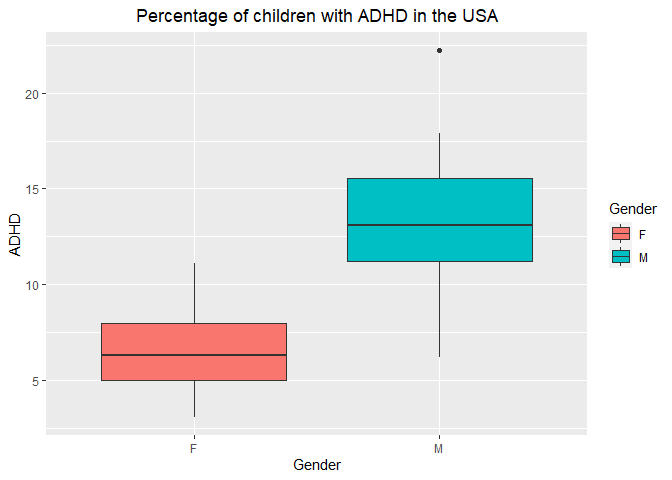
\includegraphics{datapractical_files/figure-latex/unnamed-chunk-3-1.pdf}

As we can see on the boxplot, and after realizing a t.test, the average
of boys with ADHD is significantly higher than the average of girls
(p-value \textless{} 0,05).

Then, I took data about the mean percentage of adults in the USA with
ADHD.
\href{https://www.nimh.nih.gov/health/statistics/attention-deficit-hyperactivity-disorder-adhd\#part_2553}{My
data} come from the \emph{National Institute of Mental Health}.
Unfortunately, the most recent data I could find for the USA are from
2006.

\begin{itemize}
\tightlist
\item
  \textbf{I decided to build a barplot in order to compare the mean for
  men and for women adults:}
\end{itemize}

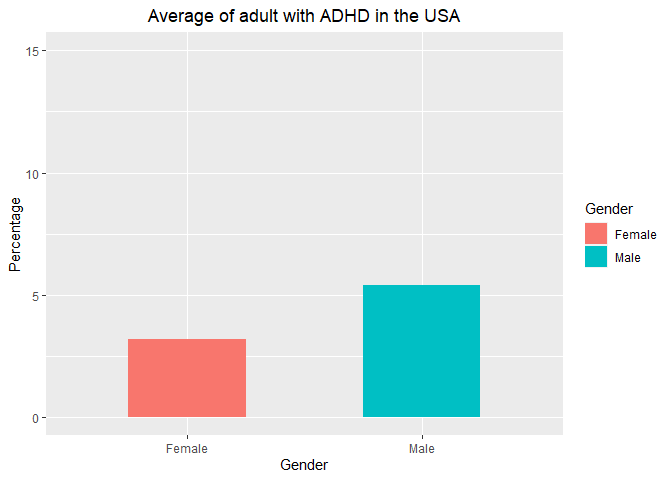
\includegraphics{datapractical_files/figure-latex/unnamed-chunk-4-1.pdf}

\begin{longtable}[]{@{}rr@{}}
\caption{Tab1. Percentage of adult with ADHD in the USA}\tabularnewline
\toprule()
Women & Men \\
\midrule()
\endfirsthead
\toprule()
Women & Men \\
\midrule()
\endhead
3.2 & 5.4 \\
\bottomrule()
\end{longtable}

This time, the t.test I realized showed no significance difference
between the men and the women percentage with ADHD. This change of
significance may goes in the direction of my hypothesis ( p-value =
0.1594).

\begin{itemize}
\tightlist
\item
  \textbf{In order to have a better visualization of mean percentage for
  children with ADHD compare to adults with ADHD, I decided to group the
  barplots.}
\end{itemize}

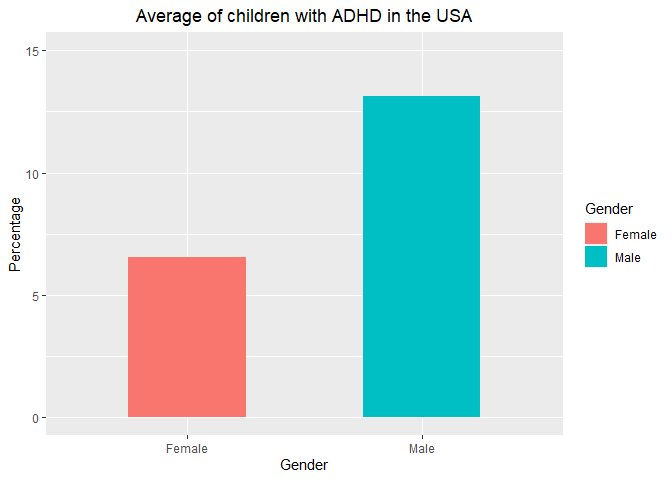
\includegraphics{datapractical_files/figure-latex/unnamed-chunk-6-1.pdf}
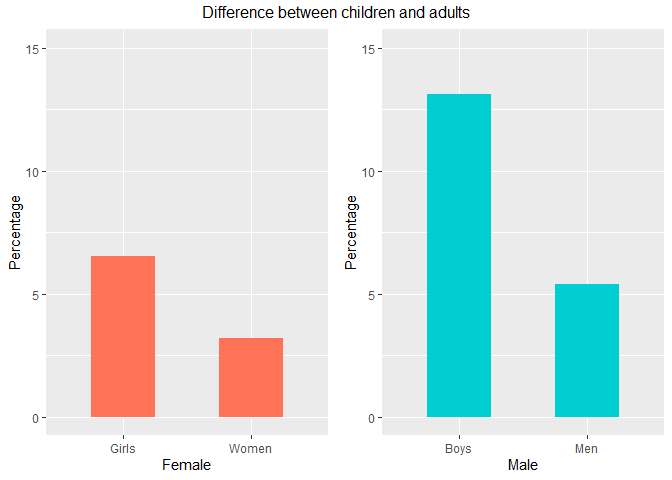
\includegraphics{datapractical_files/figure-latex/unnamed-chunk-6-2.pdf}

\begin{longtable}[]{@{}rrrr@{}}
\caption{Tab2. Average population with ADHD}\tabularnewline
\toprule()
Female & Male & Girls & Boys \\
\midrule()
\endfirsthead
\toprule()
Female & Male & Girls & Boys \\
\midrule()
\endhead
3.2 & 5.4 & 6.55 & 13.13 \\
\bottomrule()
\end{longtable}

\begin{longtable}[]{@{}ll@{}}
\caption{Tab3. Percentage of adults who still have ADHD}\tabularnewline
\toprule()
Women & Men \\
\midrule()
\endfirsthead
\toprule()
Women & Men \\
\midrule()
\endhead
\textasciitilde{} 49\% & \textasciitilde{} 43\% \\
\bottomrule()
\end{longtable}

As I said previously, it is estimated that 15 to 65 \% of children will
still have ADHD while growing up.\\
On the last table, we can see that we still have an average of 49\% of
6.55 \% of girls who still have ADHD while growing up. For the men we
have a bit less than this average, since around 43\% of the 13.13\% of
boys with ADHD will still have the disorder as an adult. I also realized
a t.test which showed no significance for this difference of percentage
between male and female (p-value = 0.4473). Both 43\% and 49\% are in
the expected results of children who would keep the disorder in
adulthood.

\hypertarget{results}{%
\subsection{Results}\label{results}}

\begin{itemize}
\tightlist
\item
  \textbf{If we recap:}
\end{itemize}

\begin{longtable}[]{@{}lll@{}}
\caption{T.test for significance}\tabularnewline
\toprule()
For children & For adults & For children vs adults \\
\midrule()
\endfirsthead
\toprule()
For children & For adults & For children vs adults \\
\midrule()
\endhead
p-value \textless{} 2.2e-16 & p-value = 0.1594 & p-value = 0.4473 \\
\bottomrule()
\end{longtable}

There is only one significant difference for the percentage of boys and
girls diagnosed with ADHD. The fact that there isn't significant
difference among adult might go on the same direction as my hypothesis.
Moreover, the higher percentage of girls who might keep ADHD while
growing up comparing to the one for boys slightly supports my
hypothesis. However, my hypothesis is not supported in a very reliable
way as there is no significant difference between these two percentages.

Furthermore, I couldn't find data for both adults and children from the
same year of survey and the research about ADHD are increasing such as
awareness. Therefore, my results aren't very reliable since I might not
be comparing the same proportion of percentage in the actual population.

\hypertarget{conclusion}{%
\subsection{Conclusion}\label{conclusion}}

AS I said my previously my results aren't very reliable. However, it
seems that girls still have a higher rate of deleyed diagnosis which can
be very impactful in their life. Actually, an early diagnosis in
childhood allows for the development of a treatment plan and strategies
to deal with everything that ADHD entails (for example organization
problem, focus, school tasks etc.). As a matter of facts, an diagnosed
and not treated ADHD higher the risk of developing comorbidities such as
anxiety, psychological distress, depression and low self-esteem (Quinn,
2005). It also often leads to social relationship impairs,
school/working failure, general demoralization and increase the risk of
consuming drugs or alcohol (Quinn, 2005). This not only impacts women
but also threatens public health. Indeed, untreated/undiagnosed women
tend to be less able to be consistent parents and less able to manage
their job and private life. In addition, the anxiety and stress
resulting from all these struggles can cause several important deceases
(Quinn, 2005).

For all the reasons I have mentioned in this paper, awareness about ADHD
is very important in order to increase the number of diagnoses and not
to forget anyone that could suffer in silence. Finally, as Dvorksy and
Langberg (2016) suggest, ``it may be preferable to ensure that (a)
diagnostic items reflect both male- and female-specific manifestations,
(b) subtle indicators of inattention/disorganization are probed, and (c)
clinicians inquire about such factors as compensatory behaviors and life
transitions in girls and women.''

\hypertarget{references}{%
\subsection{References}\label{references}}

\hypertarget{articles}{%
\subsubsection{Articles:}\label{articles}}

Dvorsky, M.R., Langberg, J.M. (2016). A Review of Factors that Promote
Resilience in Youth with ADHD and ADHD Symptoms. \emph{Clin Child Fam
Psychol Rev} 19, 368--391.

Heidbreder R. (2015). ADHD symptomatology is best conceptualized as a
spectrum: a dimensional versus unitary approach to diagnosis.
\emph{Attention deficit and hyperactivity disorders}, 7(4), 249--269.

Katzman, M.A., Bilkey, T.S., Chokka, P.R. \emph{et al.} (2017). Adult
ADHD and comorbid disorders: clinical implications of a dimensional
approach. \emph{BMC Psychiatry} 17, 302.

Purper-Ouakil, D., Ramoz, N., Lepagnol-Bestel, AM. \emph{et al.} (2011).
Neurobiology of Attention Deficit/Hyperactivity Disorder. \emph{Pediatr
Res} 69, 69--76.

Quinn, P., Wigal, S. (2004). Perceptions of girls and ADHD: results from
a national survey. \emph{MedGenMed} 6(2):2.

Quinn, P.O. (2005). Treating adolescent girls and women with ADHD:
Gender-Specific issues. \emph{J. Clin. Psychol.}, 61: 579-587.

\hypertarget{data-1}{%
\subsubsection{Data:}\label{data-1}}

\begin{itemize}
\tightlist
\item
  National Institute of Mental Health, from:

  \begin{itemize}
  \tightlist
  \item
    Kessler, R. C., Adler, L., Barkley, R., Biederman, J., Conners, C.
    K., Demler, O., Faraone, S. V., Greenhill, L. L., Howes, M. J.,
    Secnik, K., Spencer, T., Ustun, T. B., Walters, E. E., \& Zaslavsky,
    A. M. (2006). The prevalence and correlates of adult ADHD in the
    United States: results from the National Comorbidity Survey
    Replication. \emph{The American journal of psychiatry}, 163(4),
    716--723.

    \begin{itemize}
    \tightlist
    \item
      \href{https://www.nimh.nih.gov/health/statistics/attention-deficit-hyperactivity-disorder-adhd\#part_2553}{Data
      table}.
    \end{itemize}
  \end{itemize}
\item
  Child and Adolescent Health Measurement Initiative. 2020-2021 National
  Survey of Children's Health (NSCH) data query. Data Resource Center
  for Child and Adolescent Health supported by the U.S. Department of
  Health and Human Services, Health Resources and Services
  Administration (HRSA), Maternal and Child Health Bureau (MCHB).
  Retrieved from \url{https://mchb.hrsa.gov/data/national-surveys}

  \begin{itemize}
  \tightlist
  \item
    \href{https://www.childhealthdata.org/browse/survey/allstates?q=9343\&g=1008\&a=18062\#}{Data
    table}
  \end{itemize}
\end{itemize}

\hypertarget{pictures}{%
\subsubsection{Pictures:}\label{pictures}}

\begin{itemize}
\tightlist
\item
  {[}@ADHD\_couple{]}.(2020, October 4).Retrieved on
  \href{https://www.instagram.com/p/CF7aB2NDL3j/?hl=f}{Instagram}
\end{itemize}

\end{document}
